\documentclass[12pt]{article}

\usepackage{algorithm}
\usepackage{amsmath}
\usepackage{float}
\usepackage[letterpaper]{geometry}
\usepackage{graphicx}
\usepackage{hyperref}
\usepackage{pdfx}
\usepackage{listings}
\usepackage{pdflscape}

\begin{document}

\title{Evaluating the performance of extending Booth's algorithm}
\author{Adam Gausmann}
\date{21 March 2022}
\maketitle

\section*{Abstract}

Booth's algorithm is a multiplication algorithm often favored for its
simple hardware while still providing decent performance, by looking ahead at 2
bits per iteration. However, it may not be the best option in that regard; it
might be possible to get better performance in a similar size by extending the
same technique, looking ahead at 3 or 4 bits, but these extensions do require
additional hardware.

In this paper we analyze this size/performance tradeoff, by formalizing these
extended algorithms, constructing a practical hardware model to determine the
timing of the algorithms, and developing a simulator to empirically analyze
their execution time for a selection of word sizes.

Based on our model, the 4-bit version of Booth's algorithm shows noticeable
improvements in performance for input words of at least 8 bits, but there are
clearly diminishing returns compared to the increased hardware complexity.

\newpage

\section{Introduction}

\subsection{Background}

Multiplication is a very common operation in computing; it is used in low-level
routines like calculating offsets in an array, and it is also present in many
higher-level algorithms. While it can be emulated in software using very little
memory and simple operations like add and shift, hardware multipliers offer
much better performance and often can significantly improve the overall
execution time of programs. Because of this, hardware multipliers are included
in most general-purpose processor designs. Multiplication is very
parallelizable at the bit level in hardware using reduction of summands;
however, the hardware required grows quadratically with the word size. For
example, a multiplier for two 64-bit factors would need 4096 AND gates just to
generate the matrix of summands! Because of this, sequential algorithms like
add-and-shift still have some use in hardware implementations.  However, we can
do better than a simple add-and-shift, and that is the basis for Booth's
algorithm.

The fundamental idea of add-and-shift is to iterate through the bits of one
factor, one bit at a time, and to add the other factor to the output register
whenever a 1 is encountered. Booth's algorithm extends this concept by
looking at the least significant 2 bits at a time and making a decision whether
it needs to add \textit{and} what term to add. When matching against 2 bits
there are four cases to consider, and the decision table for Booth's algorithm
looks like this:

\vspace{12pt}
\begin{tabular}{|r|l|}
    \hline
    00 & Shift right 1. \\
    01 & Add $A$ to output and shift right 1. \\
    10 & Subtract $A$ from output and shift right 1. \\
    11 & Shift right 1. \\
    \hline
\end{tabular}
\vspace{12pt}

\subsection{Generalizing Booth's Algorithm}

Booth's algorithm can be modified to an even more general case, to look at $k$
bits and shift by $k - 1$ bits on each iteration. The tables for values of $k$
greater than 2 can be found by considering how the bit patterns would be
interpreted when $k = 2$. For example, the bit pattern 0110 in $k = 4$ is the
same as the bit patterns 10, 11, and 01\footnote{If this seems backwards,
remember that Booth's algorithm looks at the least significant bits on each
iteration and then performs a right shift.}
in $k = 2$, which would result in the steps:

\begin{enumerate}
    \item Add $A$ and shift right 1.
    \item Shift right 1.
    \item Subtract $A$ and shift right 1.
\end{enumerate}

By reordering the subtraction before the shifts, it can be simplified to add
$A$, subtract $4A$, and shift right 3. So, the net effect of this pattern is to
subtract $3A$ at the current position.

\subsection{Motivation}

For Booth's algorithm, the advantage over add-and-shift is that on average,
less additions and subtractions are needed, improving the average execution
time. ``Modified'' Booth's algorithm, where $k > 2$, offers the potential for
even better execution time by performing fewer iterations. The total number of
iterations is reduced by a factor of approximately $k-1$; however, the lookup
table grows exponentially and its values become more complex to precompute. In
practice, $k=4$ is typically the highest feasible value, and often $k=3$ or
$k=2$ will be more optimal.

The focus of this paper is to evaluate the performance of this modified version
of Booth's algorithm, focusing on the application of $k=3$ and $k=4$ to some
relatively small word sizes of 4, 6, 8, 10, and 12 bits.

\section{Methods}

The modified Booth's algorithms were first formalized in pseudocode, which was
used to create a practical hardware design. Then, a simulator was developed
that closely follows the pseudocode and tracks the execution time of the
circuit.

\subsection{Formulation of Modified Booth}

The 3-bit and 4-bit extended versions of Booth's algorithm are provided as
pseudocode in Algorithms \ref{alg:booth3} and \ref{alg:booth4}. Between them,
the overall structure is similar, but there are some differences where the
algorithm depends on the group size, specifically: the number of iterations
(step 3), the shift amounts (steps 5, 7, and 10), and the decision table (step
6).

\begin{algorithm}[H]
    \begin{lstlisting}
Booth3(A, B, n):
    1. Shift B left, inserting zero for LSB.
    2. Let PQ = 0 (double register).
    3. Let m = ceil((n + 1) / 2).
    4. Let k = 0.
    5. Shift PQ right 2 bits, preserving sign.
    6. Match against the lower 3 bits of B:
        000 or 111 => no action.
        001 => Add 1*A to P.
        010 => Add 1*A to P.
        011 => Add 2*A to P.
        100 => Subtract 2*A from P.
        101 => Subtract 1*A from P.
        110 => Subtract 1*A from P.
    7. Shift B right 2 bits, preserving sign.
    8. Increment k.
    9. If k < m, repeat from step 5.
    10. Shift PQ right (n mod 2) bits, preserving sign.
    11. Return the contents of PQ.
    \end{lstlisting}
    \caption{Pseudocode to describe 3-bit Booth's algorithm.}
    \label{alg:booth3}
\end{algorithm}
\newpage

\begin{algorithm}[H]
	\begin{lstlisting}
Booth4(A, B, n):
    1. Shift B left, inserting zero for LSB.
    2. Let PQ = 0 (double register).
    3. Let m = ceil((n + 1) / 3).
    4. Let k = 0.
    5. Shift PQ right 3 bits, preserving sign.
    6. Match against the lower 4 bits of B:
        0000 or 1111 => no action.
        0001 => Add 1*A to P.
        0010 => Add 1*A to P.
        0011 => Add 2*A to P.
        0100 => Add 2*A to P.
        0101 => Add 3*A to P.
        0110 => Add 3*A to P.
        0111 => Add 4*A to P.
        1000 => Subtract 4*A from P.
        1001 => Subtract 3*A from P.
        1010 => Subtract 3*A from P.
        1011 => Subtract 2*A from P.
        1100 => Subtract 2*A from P.
        1101 => Subtract 1*A from P.
        1110 => Subtract 1*A from P.
    7. Shift B right 3 bits, preserving sign.
    8. Increment k.
    9. If k < m, repeat from step 5.
    10. Shift PQ right (n mod 3) bits, preserving sign.
    11. Return the contents of PQ.
	\end{lstlisting}
    \caption{Pseudocode to describe 4-bit Booth's algorithm.}
    \label{alg:booth4}
\end{algorithm}
\newpage

\subsection{Simulator}

The simulator has been developed as a Rust library providing the
\texttt{booth3} and \texttt{booth4} functions, with some command-line utilties
to help interface with these functions. The source code for the simulator is
available on GitHub at \url{https://github.com/agausmann/cpe5110-project}. See
the \texttt{README.md} file for instructions on how to run it yourself.

\subsection{Correctness}

The simulator has been exhaustively tested and confirmed to produce the correct
product on all pairs of two's complement 4-, 6-, 8-, 10-, and 12-bit values.
For the exact testing procedure used, see \texttt{tests/exhaustive.rs} in the
simulator's source code.

To prove that the algorithm itself is correct, it can be shown that it behaves
identically to the original Booth's algorithm which is assumed correct.  For
$PQ$ to be the same value in original and modified Booth's algorithm, it has to
be shifted the same number of times, and the decision steps have to be
equivalent.

Since the decision table for modified Booth's algorithm on $k$ bits is
explicitly constructed from the $k - 1$ decisions that would be made by the
original Booth's algorithm, then each stage in modified Booth's algorithm is
equivalent to exactly $k - 1$ stages in the original Booth's algorithm. Those
original decisions also correspond to $k - 1$ 1-bit shifts, which are
equivalent to a single $k - 1$ bit shift. After this stage, the next stage in
modified Booth's algorithm continues at exactly the same position that the
original algorithm is also continuing from. This repeats until all bits of $B$
are consumed.

There is an edge case that has to be considered when the number of bits $n$
isn't divisible by $k$. In that case, on the last iteration of modified Booth's
algorithm, only $n\mod k$ bits will be from $B$, and the remaining $k - (n\mod k)$
are extra bits that weren't originally part of $B$. If that group is
interpreted as the decisions that the original Booth's algorithm would make,
there are an extra $k - (n\mod k)$ decisions. However, since the right shift of
$B$ is sign-preserving, these bits are equal to the sign bit (most significant
bit) of the original value of $B$, and so all of the extra patterns are 00 or
11 which do not affect the value of $PQ$.

Those extra 00 and 11 patterns would also correspond to extra shifts, but these
shifts are not performed. After the last iteration, the final shift is $n\mod
k$ (pseudocode line 10), which corresponds to the number of bits remaining from
the original value of $B$.

Therefore, modified Booth's algorithm executes in lock-step with the original
Booth's algorithm, and so it produces an equivalent result.

\section{Results}

\subsection{Timing Analysis}

\begin{figure}
    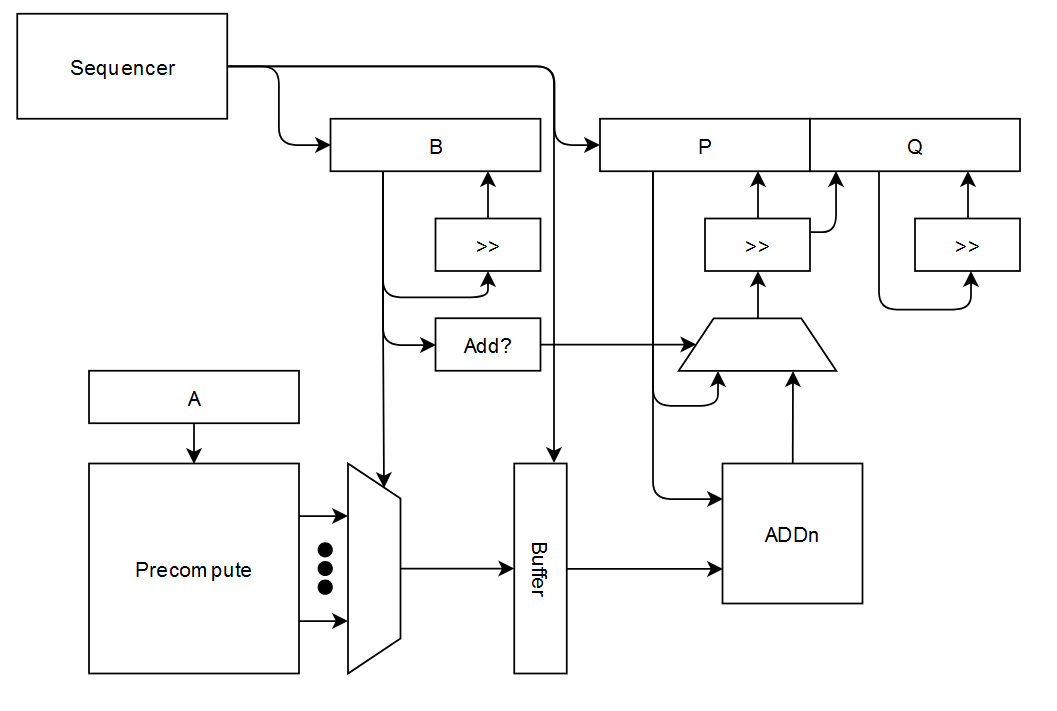
\includegraphics[scale=0.5]{booth-circuit.png}
    \caption{
        A high-level block diagram of a hardware implementation of Booth's
        algorithm and its variants.
    }
    \label{fig:booth-circuit}
\end{figure}

To analyze the performance of modified versions of Booth's algorithms, a
high-level circuit design was created with enough detail to determine the
critical path, shown in Figure~\ref{fig:booth-circuit}.

There are a few basic circuit elements whose timings are given, which will be
used in the following analysis:

\begin{itemize}
    \item Two's complement of an $n$-bit value takes $n\Delta t$;
    \item Latching takes $3\Delta t$;
    \item An $n$-way multiplexer takes $(\lceil \log_2{n}\rceil + 1)\Delta t$
        (if the maximum gate fan-in is 2);
    \item The adders used are carry-select, whose delay will be denoted as
        $CS_n$ for an $n$-bit adder. The exact values used for $CS_n$ in this
        simulation are presented and justified in
        Appendix~\ref{app:carry-select-timing}.
\end{itemize}

There is some setup time required, equivalent to the delay needed to precompute
the table, determine the first addend, and buffer it:

\begin{itemize}
    \item For $k = 3$, the longest precomputation is $-2A$, a bit shift and a
        complement that takes $n\Delta t$. With 6 cases, the 6-way multiplexer
        takes $4\Delta t$. Finally, the buffer takes $3\Delta t$ to latch. So,
        the total setup time is $(n + 7)\Delta t$.

    \item For $k = 4$, the longest precomputation is $-3A$, which can be
        accomplished with an $n$-bit carry-select adder and a complement that
        takes $CS_n + n\Delta t$. The 14-way
        multiplexer takes $5\Delta t$, and the buffer still takes $3\Delta t$.
        So the total setup time is $CS_n + (n + 8)\Delta t$.
\end{itemize}

On each iteration, two things can potentially happen: a lookup from the
precomputed table, and an addition. Although the addition depends on the result
of the lookup, it can be pipelined by buffering the result of the lookup, and
performing the lookup for the next iteration while performing the addition for
the current iteration.

During iteration, the data loop out of and into $PQ$ can either take $2\Delta
t$ if no addition is needed, or $CS_n + 2\Delta t$ if addition is performed. At
the same time as the $PQ$ calculation, the lookup for the next group of bits is
being performed, which will be $(k + 1)\Delta t$ for the multiplexer.  So, the
effective delay on each iteration is either $\max(2\Delta t, (k + 1)\Delta t)$,
or $\max(CS_n + 2\Delta t, (k + 1)\Delta t)$ depending on whether addition was
performed.

\subsection{Simulation Results}

\begin{figure}
    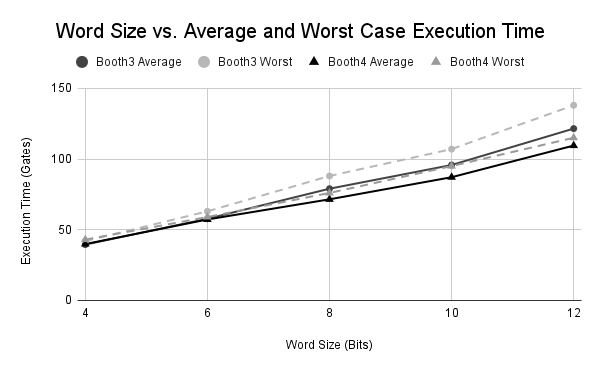
\includegraphics[scale=0.6]{delay-averages.png}
    \caption{
        Average and worst-case execution time of both 3-bit and 4-bit Booth's
        algorithm, aggregated by word size. These values are calculated over
        the whole n-bit input space of the multiplier, and the averages are
        unweighted.
    }
    \label{fig:delay-averages}
\end{figure}

The simulation was run on two datasets. The first one was a small set of values
designed to check for accuracy and certain timing patterns; that table can be
found in Appendix~\ref{app:results-table}. The simulation was also run
exhaustively across the entire range of possible imputs to analyze the average
and worst-case execution times for each word and group size; these results are
presented in Figure~\ref{fig:delay-averages}.

As shown in Figure~\ref{fig:delay-averages}, when the word size is 4 or 6 bits,
there is no significant difference in performance between 3-bit and 4-bit
modified Booth's. When the word size is 8 bits or higher, 4-bit Booth's shows a
measurable improvement, approximately 10\% speedup for both average and
worst-case.

\section{Conclusion}

4-bit modified Booth's has been shown to improve performance compared to 3-bit
in some scenarios, but it doesn't scale perfectly. The number of iterations is
reduced from $\lceil\frac{n + 1}{2}\rceil$ to $\lceil\frac{n + 1}{3}\rceil$,
but simultaneously, the probability that additions will be skipped on each
iteration is halved, from $\frac{2}{8}$ to $\frac{2}{16}$.

These improvements also come at a cost; the hardware for the 4-bit algorithm is
roughly twice as complex as for 3-bit. If cost and size are not a major
concern, then it may be worth implementing 4-bit for the performance
improvements.

It is also worth noting that these performance results are just a first-order
approximation, based on a timing analysis in an idealized model. As such, they
might not account for all of the physical limitations present in a hardware 
design. These limitations could be addressed in future work by improving the
simulation to be more physically-accurate.

Multiplication is a complex algorithm that humanity has spent millenia trying
to optimize. Unfortunately there is no one ``best'' algorithm; they all have
different strengths, and which algorithm to choose largely depends on what
technologies are available for the implementation. Booth's algorithm and its
variants generally perform well in digital hardware, and are a decent
compromise between the performance of reduction schemes and the simplicity of
add-and-shift.

\newpage
\appendix

\section{Timing Analysis of Carry-Select Adders}
\label{app:carry-select-timing}

For this simulation, we assumed that all adders are optimal carry-select
adders. Here are the propagation delays $CS_n$ used in the simulation, along
with their optimal ``topologies,'' whose definition will follow:

\vspace{12pt}
\begin{tabular}{|r|r|l|}
    \hline
    $n$ & $CS_n$ & Topology \\
    \hline
    4 & $8\Delta t$ & 2-2 \\
    6 & $10\Delta t$ & 3-3 \\
    8 & $12\Delta t$ & 4-4 \\
    10 & $12\Delta t$ & 4-3-3 \\
    12 & $14\Delta t$ & 4-4-4 \\
    \hline
\end{tabular}
\vspace{12pt}

For this analysis, we consider the ``topology'' of a carry-select adder to be
defined as $m$ ``groups'' of bits, where each group size is $n_m$ through
$n_1$. For example, a 2-2 carry-select adder has two groups ($m = 2$), each with
two bits ($n_2 = 2$ and $n_1 = 2$).

To construct a carry select adder, for the first group of $n_1$ bits, use a
$n_1$-bit ripple-carry adder. For all remaining groups, $n_k$ where $1 < k \le
m$, use a ``select module'' on $n_k$ bits. Connect the carry-out of the
ripple-carry adder to the carry-in of the first select module, and connect the
carry-out of every select module except for the last one to the carry-in of the
next one, so you end up with a circuit like this:

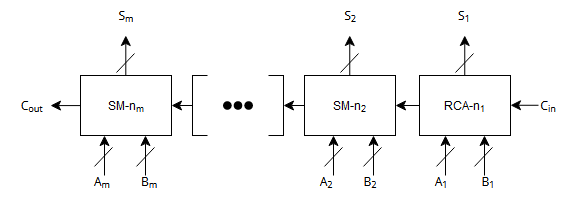
\includegraphics{carry-select.png}

The $n$-bit ``select module'' is composed of two $n$-bit ripple-carry adders
with their carry inputs hardwired to zero and one, whose sum and carry-out are
multiplexed using the module's carry-in to produce the module's sum and
carry-out:

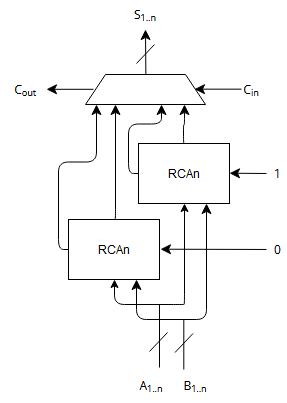
\includegraphics{select-module.png}

Finally, a ripple-carry adder is the typical design: collection of 1-bit full
adders whose carries are chained.

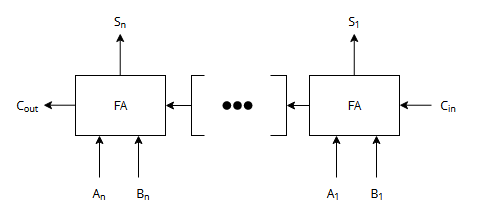
\includegraphics{ripple-carry.png}

The sum and carry-out of all $n$-bit ripple-carry adders in this design is
generated in $2(n + 1)\Delta t$.

When calculating the delay for a select module, first determine which is
larger: the delay for its own ripple-carry adders, or the delay on its
carry-in. Then, add the multiplexer's delay (assumed to be $2\Delta t$) to that
value.

Finally for the whole carry-select adder, the delay of its output is the delay
of the leftmost select module.

This algorithm is implemented as a Python function which takes
the group sizes as a list, which was used to generate the table:

\lstinputlisting[language=python]{carry_select_delay.py}

As an example, a 4-3-3 carry select adder should have a delay of 12:

\begin{lstlisting}[language=python]
>>> from carry_select_delay import carry_select_delay
>>> carry_select_delay([4, 3, 3])
12
\end{lstlisting}

\begin{landscape}
    \section{Simulation Results Table}
    \label{app:results-table}

    These are the results of running simulations on the given test data. I, A,
    and T are the number of iterations, number of additions and subtractions,
    and execution time (in terms of $\Delta t$) respectively.

    \vspace{12pt}
    \begin{tabular}{ |rrr|rr|rrr|rrr| }
        \hline
        Multiplier & Multiplicand & Bits & \multicolumn{2}{|c|}{Product} & \multicolumn{3}{|c|}{Booth3} & \multicolumn{3}{|c|}{Booth4}  \\
        (binary) & (binary) & & (binary) & (hex) & I & A & T & I & A & T \\
        \hline
        1110 & 1111 & 4 & 00000010 & 02 & 3 & 1 & 37 & 2 & 1 & 38 \\
        0101 & 0101 & 4 & 00011001 & 19 & 3 & 2 & 42 & 2 & 2 & 43 \\
        \hline
        111111 & 111111 & 6 & 000000000001 & 001 & 4 & 1 & 49 & 3 & 1 & 52 \\
        101110 & 110111 & 6 & 000010100010 & 0a2 & 4 & 2 & 56 & 3 & 2 & 59 \\
        111011 & 100011 & 6 & 000010010001 & 091 & 4 & 2 & 56 & 3 & 2 & 59 \\
        \hline
        00011111 & 01010101 & 8 & 0000101001001011 & 0a4b & 5 & 2 & 70 & 3 & 2 & 67 \\
        11010111 & 01010101 & 8 & 1111001001100011 & f263 & 5 & 4 & 88 & 3 & 3 & 76 \\
        01010101 & 11010111 & 8 & 1111001001100011 & f263 & 5 & 4 & 88 & 3 & 3 & 76 \\
        01110111 & 00110011 & 8 & 0001011110110101 & 17b5 & 5 & 4 & 88 & 3 & 3 & 76 \\
        01111000 & 01110111 & 8 & 0011011111001000 & 37c8 & 5 & 2 & 70 & 3 & 2 & 67 \\
        \hline
        0101010101 & 0101010101 & 10 & 00011100011000111001 & 1c639 & 6 & 5 & 107 & 4 & 4 & 95 \\
        1100111011 & 1001110000 & 10 & 00010011001111010000 & 133d0 & 6 & 4 & 98 & 4 & 3 & 86 \\
        1001101110 & 0101111010 & 10 & 11011010111001101100 & dae6c & 6 & 4 & 98 & 4 & 4 & 95 \\
        \hline
        010101010101 & 010101010101 & 12 & 000111000110111000111001 & 1c6e39 & 7 & 6 & 138 & 5 & 4 & 115 \\
        001111100111 & 000011111111 & 12 & 000000111110001100011001 & 03e319 & 7 & 4 & 116 & 5 & 3 & 104 \\
        101010101010 & 101010101010 & 12 & 000111000111100011100100 & 1c78e4 & 7 & 6 & 138 & 5 & 4 & 115 \\
        111001110000 & 000011111111 & 12 & 111111100111000110010000 & fe7190 & 7 & 3 & 105 & 5 & 3 & 104 \\
        \hline
    \end{tabular}
\end{landscape}

\end{document}
